\documentclass[12pt, a4paper]{article}
\usepackage[utf8]{inputenc}
\usepackage{amsmath}
\usepackage{amssymb}
\usepackage{natbib}
\usepackage{mathtools}
\usepackage{titling}
\usepackage[hidelinks]{hyperref}
\usepackage{booktabs}
\usepackage{float}
\usepackage{pbox}
\usepackage{adjustbox}
\usepackage{MnSymbol}
\usepackage{wasysym}
\usepackage{geometry}
\usepackage[font={it}, labelfont=bf]{caption}
\usepackage{graphicx}

%\usepackage{setspace}
%\doublespacing

\graphicspath{ {images/} }

\author{Reid McIlroy-Young}
\title{An Novel RNN Approach to Classification of Complex Textual Scientific Metadata \\ \quad \\ \large MACS 30200 Final Paper}
\date{June 4, 2017}

\setcounter{tocdepth}{2}

\begin{document}
\pagenumbering{Roman}
\maketitle
\begin{abstract}
	\thispagestyle{plain}
	\textit{
		We 
	}
\end{abstract}		
\newpage
\tableofcontents
%\listoffigures
%\listoftables

\newpage
\setcounter{page}{1}
\pagenumbering{arabic}

\section{Introduction}



\section{Literature Review}

Computer's have been a formal part of scientific work since the 18th Century \citep{grier2013computers}, but the modern day electromechanical machines developed by Turing \citep{turing1937computable} and many others \citep{abbate2012recoding}\citep{abbate2000inventing} are a much more recent innovation, of the last century \citep{bauer1972software}.  The introduction of these devices to communities around the world (both metaphorically and literally) has had major impacts on the culture \citep{lessig2007code}, technology\citep{abbate2000inventing} and rate of development \citep{bauer1972software}. Much work has been done to study these effects, but it has been primarily focused on either the macro cultural effects \citep{pfaffenberger1988social} or the economic/business usage \citep{landauer1995trouble}. 

By comparison the usage of computers by scientists has been overlooked by researchers \citep{sloanrep}. This oversight has many reasons, but one of the most significant is the lack of available data. The primary methods for large scale analysis of the culture or structure of scientific work involve bibliometric techniques \citep{de2009bibliometrics} using large standard datasets\citep[e.g.][]{Boyack2005, borner2010atlas, borner2015atlas, sugimoto2013global, shi2015weaving, evans_meta, skupin2013visualizing}. These dataset are generally lacking information about the computational aspects of the work, e.g. the  Clarivate Analytics Web of Science (WOS) does not have any such field \citep{mkdocs} and as such research into this dimension is difficult. Recent developments in natural language processing (NLP) have shown that complex concepts can be extracted reliably from text for a wide variety of tasks \citep{evans2016machine}, with some very similar to that done here \citep{foster2015tradition}.

\subsection{Information Extraction}

To extract the information about software usage from the available data requires complex NLP techniques and the best methodologies change quickly\citep{evans2016machine}. As we are primarily concerned with the classification of meta-data for a record relating it to a new software tool or not, in theory there are a large number of available techniques, as this is a simple binary classification problem \citep{james2013introduction}\citep{jurafsky2000speech}\citep{murphy2012machine}. We have considered most of the available techniques:

\begin{itemize}
\item Classified based on a simple regular grammar, e.g. regex
\item Word collocation frequencies \citep{manning1999foundations}
\item Term frequency–inverse document frequency vectors with an SVM or other classifier \citep{collobert2011natural}
\item Word2Vec vectors with an SVM or other classifier\citep{mikolov2013distributed}\citep{collobert2011natural}
\end{itemize}

The the current state of the art for natural language processing is the usage of deep neural networks for information extraction requiring more than simple word level similarities\citep{manning-EtAl}. As this is the state of the art there is no simple set of rules to follow, but there are some guidelines \citep{Goodfellow-et-al-2016}. These have lead us to the use of a recurrent neural network (RNN) \citep{mikolov2010recurrent} for the classification, although the exact specifics have been determined with cross-validation techniques \citep{james2013introduction}. The main features to consider are the type of regularization \citep{Goodfellow-et-al-2016}, what representation of words to use (most likely Word2Vec \citep{mikolov2013distributed}), what non-textual data will be included as there are in the WOS data set over 60 possible fields for each record \citep{mkdocs} and what values the hyperparameters take\citep{Goodfellow-et-al-2016}. This tuning is highly specific to the data, framework (in this case TensorFlow \citep{abadi2016tensorflow}) and model and the parameters are provided in the supporting material.

\subsection{Data Analysis}

Once the records with new software tools have been identified, we can use the existing theory of bibliometrics to look at the network structure. The literature standard approaches are to look at the structure of these nodes in the citation and authorship graphs \citep{de2002pattern}\citep{lariviere2006canadian}\citep{borgatti2009network}. This can be a computationally intensive task but tools exists that make it more practical \citep{mclevey2017introducing} so once the records have been labelled the analysis techniques are no longer novel.

The literature is silent on basic features of scientific software usage, and even when limited to only new releases there is no existing data. Thus simple measures such as per domain counts/frequencies and basic graph measurements such as the centrality will be new contributions. 

The other main question of what causes tools to be successful, has not been answered for scientists. There has been some work in the business domain \citep{xin2008software}\citep{hsu2009computer}. The adoption of new tools by businesses is theorized to follow a sigmoid pattern, with successful new entrants having three stages of usage: First they are used by early adopters and have small market penetration. Then they reach a "take off point" and the large majority of users will adopter their tools. Finally there will be slow growth in adoption again as only the laggards are left as new users \citep{xin2008software}. This is based on adopters having a Gaussian distributed chance of adopting the tool and notably this diffusion model does not require that the software have any costs for the users and allows for network effects, thus this signature is considered in our modelling.

There also has been work done examined open source projects \citep{mockus2002two} which agrees with the theory \citep{raymond1999cathedral} of open source that success is derived from openness and collaboration. This would predict that successful tools would come from highly connected groups who are working successfully with the community. This may show up as high connectedness in the co-authorship network correlating with success.

What leads to success has also be been studied in the context of ideas in the scientific literature \citep{acharya2004ideas} \citep{johntalk} or of individuals\citep{sinatra2016quantifying}. In both cases the main measure of success is the cumulative count of citations, which we can also examine on a per paper and a per author basis. We can look for the predictors of success for a new software tool by examining its citations over time and us this as our measurement for the signature. Notably \cite{sinatra2016quantifying} show a that success very unpredictable and can happen years after the paper is published. If the software records have patterns matching this model then the diffusion model may not be a good fit.

\section{Data}

The source of data used for this analysis is the  Web of Science (WOS) database hosted by Knowledge Lab. It has metadata on almost all scientific publications from 1960 to 2015, with new records being more complete. Each publication can be linked to one or more other tables each which contain other metadata than the main table, the number of entries for each table I am concerned with are shown in Table \ref{wos} and the complete database schema in Figure \ref{schema}. Access to the database is controlled by Knowledge Lab so they would need to be contacted to access it, once access rights are obtain the database is found at \href{wos2.cvirc91pe37a.us-east-1.rds.amazonaws.com}{wos2.cvirc91pe37a.us-east-1.rds.amazonaws.com} and the documentation at \href{http://docs.cloudkotta.org/dataguide/wos.html}{http://docs.cloudkotta.org/dataguide/wos.html}.

The data for WOS were collected by Thompson Reuters until 2016, when it was given to  Clarivate Analytics who now maintain it. The contemporary publications are collected from the publishers directly while older and more obscure publications are obtained from scanned copies digitalized with OCR, which is one of the factors that leads to newer publications having much higher quality data.

\begin{table} [!ht]
	\centering
	\begin{tabular}{lr}
		\toprule
		Table & Number of Entries\\
		\midrule
		publications & 57136685\\
		abstracts &	26093439\\
		publishers & 50668193\\
		keywords &	78155603\\
		references &	1085738245\\
		\bottomrule
	\end{tabular}
	\caption{Web of Science database number of entries per table}\label{wos}
\end{table}

\begin{figure}[!ht]
	\centering
	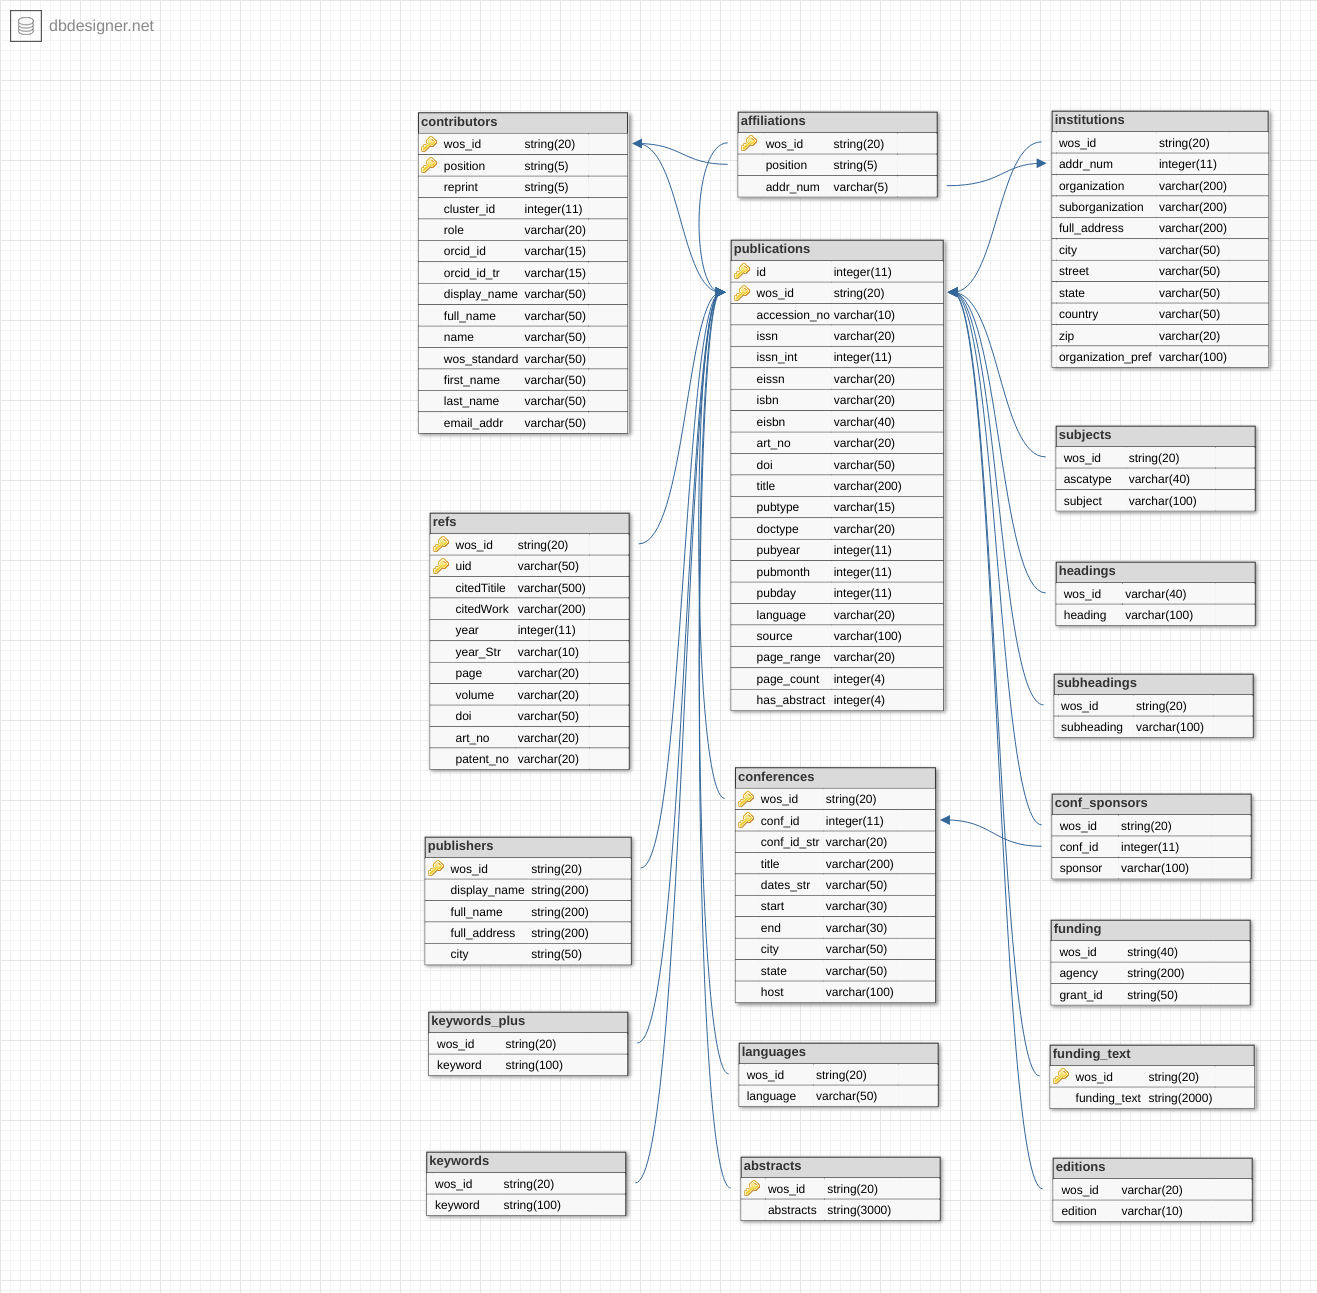
\includegraphics[width=\textwidth]{wos2_schema}
	\caption{Knowledge Lab WOS database schema}\label{schema}
\end{figure}

For this analysis I limited my data to those journals from the top 123 statistics publications between 2005 and 2016, giving me a total of 78 971 articles (publications). From these I derived a training set of classified (training) and unclassified publications. To do this I found journals that almost entirely publish new scientific software, thus all articles from these can be classified as containing new software, i.e. as positive. There are also some that contain virtually none, all of their publications can then be classified as negative.  The classified journals are given in Table \ref{journals}, note they are all top statistics journals from the data set.

\begin{figure} [H]
	\centering
	\begin{adjustbox}{center}
		\begin{tabular}{lccc}
			\toprule
			Journal & Classification & Total Citations & Impact Factor\\
			\midrule
			R JOURNAL & Mostly Software & 271 & 1.045\\
			STATA JOURNAL&Mostly Software&2636&1.292\\
			\pbox{20cm}{JOURNAL OF\\STATISTICAL SOFTWARE}&Mostly Software &6868&2.379\\
			&&&\\
			ECONOMETRICA&Little Software&24957&4.053\\
			TECHNOMETRICS&Little Software&6062&1.435\\
			\pbox{20cm}{STATISTICAL METHODS IN\\ MEDICAL RESEARCH}& Little Software &2703&4.634\\
			&&&\\
			\pbox{20cm}{JOURNAL OF THE ROYAL STATISTICAL\\ SOCIETY SERIES B-STATISTICAL METHODOLOGY} &Little Software&2 360 &1.702\\
			&&&\\
			\pbox{20cm}{BRITISH JOURNAL OF MATHEMATICAL \&\\ STATISTICAL PSYCHOLOGY}&Little Software&1 278 &3.698\\
			&&&\\
			\pbox{20cm}{ANNUAL REVIEW OF STATISTICS\\ AND ITS APPLICATION}&Little Software&74 & 3.045\\
			&&&\\
			ANNALS OF STATISTICS&Little Software&15 680 &2.780\\
			\pbox{20cm}{STOCHASTIC ENVIRONMENTAL \\RESEARCH AND RISK ASSESSMENT}&Little Software&2 297 &2.237\\
			\bottomrule
		\end{tabular}
	\end{adjustbox}
	\caption{Classified journals, citations and impact factors are both from 2015 }\label{journals}
\end{figure}

When combined the I have a training set of 1251 positive and 4362 negative examples. This is not a large data set nor is it pure since some articles from the positive set are in fact negative, one example\citep{wickham2014tidy} is shown Figure \ref{badPos}. As there is no pre-existing know set of cleaning papers I cannot give an exact count of the incorrectly identified papers, but as I will discuss later the model is capable of identifying them despite their presence in the training set. The paper used here is one of the one identified by the fully trained model as being not software. 

\begin{figure}[H]
	\begin{tabular}{ll}
		\toprule
		Field & Value\\
		\midrule
		ID & WOS:000341806800001 \\
		Source & JOURNAL OF STATISTICAL SOFTWARE \\
		Year of Publications & 2014 \\
		Title & Tidy Data \\
		Abstract &  A huge amount of effort is spent cleaning data to get it ready for\\
		&analysis, but there has been little research on how to make data\\
		&cleaning as easy and effective as possible. This paper tackles a\\
		&small, but important, component of data cleaning: data tidying. Tidy\\
		&datasets are easy to manipulate, model and visualize, and have a\\
		&specific structure: each variable is a column, each observation is a\\
		&row, and each type of observational unit is a table. This framework\\
		&makes it easy to tidy messy datasets because only a small set of\\
		&tools are needed to deal with a wide range of un-tidy datasets. This\\
		&structure also makes it easier to develop tidy tools for data\\
		&analysis, tools that both input and output tidy datasets. The\\
		&advantages of a consistent data structure and matching tools are\\
		&demonstrated with a case study free from mundane data manipulation\\
		&chores. \\
		\bottomrule
	\end{tabular}
	\caption{An example of a false positive in the training set}\label{badPos}
\end{figure}

\section{Methods}
sdffsdds
\section{Results}
dfddfs
\section{Conclusion}
dsdfsdfs
\newpage
\bibliography{Report}{}
%\bibliographystyle{plain}
\bibliographystyle{asr}

\end{document}